\documentclass[stu,12pt,floatsintext]{apa7}

%\usepackage[american]{babel}
\usepackage{enumitem}
\usepackage{array}
\usepackage{makecell} % Para permitir saltos de línea en las celdas
\usepackage{longtable}

\usepackage{caption} % Paquete para controlar los captions
\captionsetup{justification=centering, singlelinecheck=false}
\captionsetup[longtable]{justification=centering, labelsep=colon}
\captionsetup[table]{justification=centering, labelsep=colon}

%\captionsetup[longtable]{justification=centering, singlelinecheck=false} % Centra el caption de longtable

%\usepackage[justification=centering]{caption}

\usepackage{csquotes} % One of the things you learn about LaTeX is at some level, it's like magic. The references weren't printing as they should without this line, and the guy who wrote the package included it, so here it is. Because LaTeX reasons.
\usepackage[T1]{fontenc} 
\usepackage{mathptmx} % This is the Times New Roman font, which was the norm back in my day. If you'd like to use a different font, the options are laid out here: https://www.overleaf.com/learn/latex/Font_typefaces
\usepackage[spanish,es-tabla]{babel}
\setcounter{secnumdepth}{3}
\title{	Clasificación de Microservicios para un Sistema IoT enfocado en la seguridad de labores mineras en la provincia de Sugamuxi del departamento de Boyacá.}
%\authorsnames{William Fernando Salamanca Barrera, Oscar Ricardo Guerrero Serna}
\authorsnames{William Fernando Salamanca Barrera}

\authorsaffiliations{Universidad Pedagógica y Tecnológica de Colombia}
\course{Seminario de Trabajo de Grado 8108918} % LaTeX gets annoyed (i.e., throws a grumble-error) if this is blank, so I put something here. However, if your instructor will mark you off for this being on the title page, you can leave this entry blank (delete the PSY 4321, but leave the command), and just make peace with the error that will happen. It won't break the document.
\professor{PhD. Marco Javier Suarez Baron}  % Same situation as for the course info. Some instructors want this, some absolutely don't and will take off points. So do what you gotta.s

\duedate{\today}

%\abstract{Put your abstract here. In APA style, the abstract should be between 150 and 250 words depending on the journal.}
\begin{document}
	\maketitle
	\graphicspath{{./images/}}
	\renewcommand\theadset{\renewcommand\arraystretch{1.5}} % Espacio extra para encabezados
	\renewcommand\contentsname{TABLA DE CONTENIDO}
	\tableofcontents
	
	\renewcommand\listfigurename{TABLA DE FIGURAS}
	\listoffigures
	\renewcommand\listtablename{LISTA DE TABLAS}
	\listoftables
	\section{TEMA/TEMÁTICA}
	Internet de las Cosas (IoT) / IoT para el monitoreo de gases
	\begin{figure}[H]
		\centering
		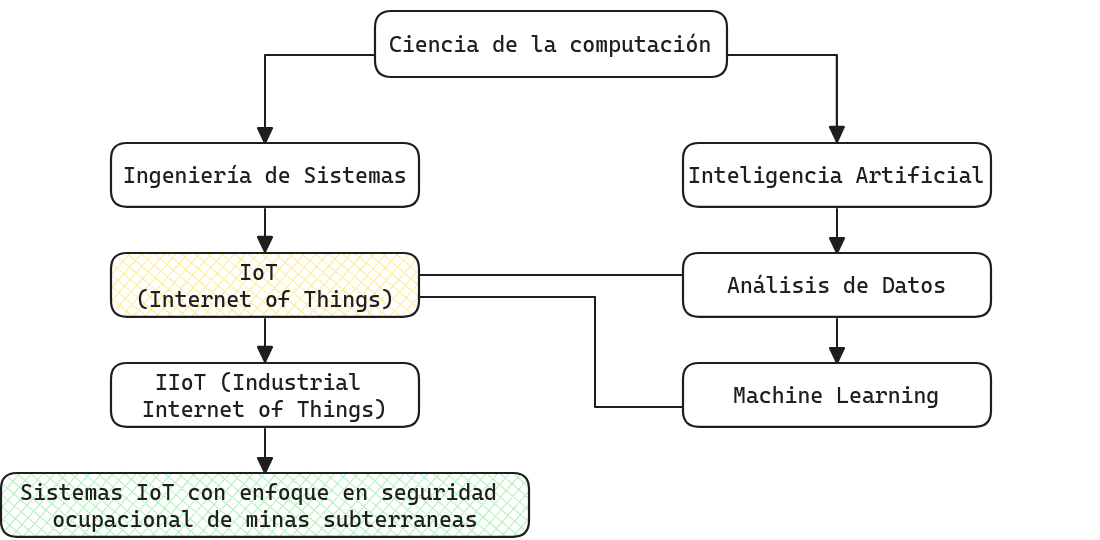
\includegraphics[scale=0.48]{mapa-conceptual}
		\captionsetup{justification=centering}
		\caption{Mapa conceptual del tema y la temática}
		\small
		Fuente: Autor
	\end{figure}
	\section{TITULO PROVISIONAL}
	Clasificación de Microservicios para un Sistema IoT de seguridad de las labores mineras en minas de la provincia de Sugamuxi del departamento de Boyacá.
	
	\section{PLANTEAMIENTO DEL PROBLEMA}
	\subsection{DESCRIPCIÓN DEL PROBLEMA}

	\subsubsection{Diagnostico}
	%Un aspecto crucial en un sistema IoT para el monitoreo de gases es la recolección de datos provenientes de diferentes sensores. Se identifica que sistemas como los SCADA (Supervisory Control and Data Acquisition), de tipo comercial con un costo económico alto y otros de uso libre, fueron concebidos bajo la arquitectura cliente-servidor, una de las menos optimas para hacer frente a las demandas actuales de un sistema IoT para el monitoreo de gases . Además de que los sistemas SCADA, en su mayoría, operan a nivel de instalación\cite{YADAV2021100433}. 
	
	 En el mercado encontramos variedad de plataformas que, a nivel de capa de aplicación, nos permiten implementar sistemas IoT\ref{table:1} . ABB Ability que es orientada a la industria minera\cite{iot-platforms} y otras de uso general, tienen una característica en común de no ser viables para su uso en el monitoreo de gases en minas de la provincia de Sugamuxi en el departamento de Boyacá, esto debido a los altos costos de estos sistemas IoT. 
	 
	Las plataformas mencionadas en la tabla\ref{table:1} hacen parte de sistemas IoT propietarios que a pesar de ser altamente maduros, no permiten su integración fácilmente con sensores, actuadores y sistemas embebidos de uso semi-industrial. Además, cuando se analiza la interoperabilidad con otros sistemas, específicamente con el objetivo de compartir información con demás departamentos, partes interesadas y módulos de analítica, se requieren mejoras que vayan alineadas con practicas modernas de IIoT \cite{iot1020029}.
	
	Adicionalmente se encuentran implementaciones IoT  que hacen uso de diferentes tecnologías de código libre con el propósito de reducir costos, como la realizada en  \cite{electronics8080822}. Pero este tipo de implementaciones IoT  de bajo costo, particularmente la anteriormente mencionada presenta el inconveniente de ser una solución incompleta específicamente en capa de aplicación, ya que no tienen el enfoque hacia el monitoreo de gases para la seguridad de labores mineras de la provincia de Sugamuxi, Boyacá.
	 
	\begin{table}
	\centering
	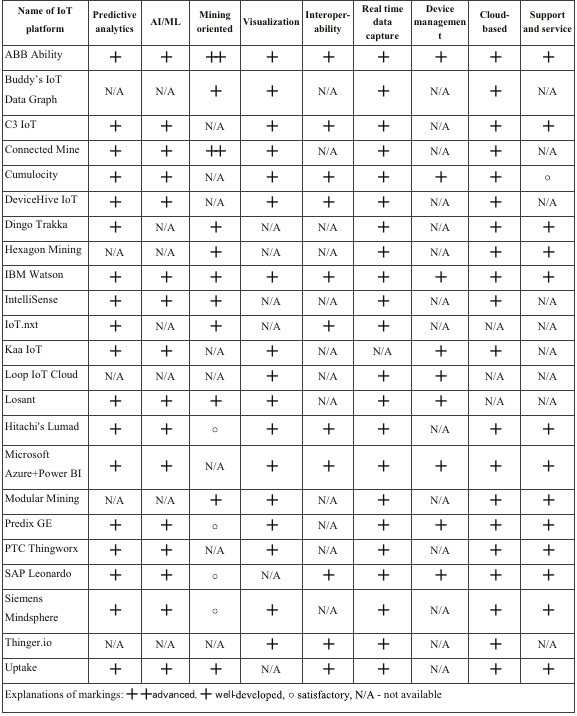
\includegraphics[scale=0.7]{plataformas-iot}
	\caption{\centering IoT platforms for the Mining Industry: An Overview\\}
	\label{table:1}
\end{table}

	\subsubsection{Pronostico}
	Optando por plataformas IoT costosas, las minas pueden empezar sufrir aumento en sus costos operativos, lo que trae una disminución de los margenes de ganancias, implicando reducción en la capacidad de re-inversión, afectando al crecimiento económico de la región con efectos como el aumento de la tasa de desempleo de los trabajadores involucrados directa e indirectamente en la cadena de producción. 
	%Además de presentarse una baja adopción en el uso de tecnología, lo cual también puede implicar que la empresa se quede resegada o hasta obsoleta frente a aquellas que si adoptan soluciones tecnológicas.
	
	Existe la posibilidad de que se opte por sistemas IoT desactualizados, la poca fiabilidad presente en algunos de estos sistemas es algo que no se puede ignorar teniendo presente el enfoque en la seguridad de las labores mineras. El uso de estándares de seguridad desactualizados, baja disponibilidad, fiabilidad e interoperabilidad, se identifican como causantes de que las partes interesadas en la seguridad de las labores mineras no puedan acceder a la información emitida por un sistema IoT desactualizado. 
	%Además cuando la demanda respecto a dispositivos conectados al sistema aumenta, nos podemos encontrar con problemas de escalabilidad que afectan la disponibilidad del sistema.
	
	En el caso de no optar directamente por un sistema IoT, no se contaría con información valiosa, principalmente en tiempo real, para la toma de decisiones en cuestiones de seguridad de las labores mineras, por lo que la seguridad de los trabajadores se ve comprometida, llevándonos a no hacer frente hacia la problemática de altos indices de accidentalidad y mortalidad minera en el departamento de Boyacá\cite{anm2020}.
		\begin{figure}[H]
		\centering
		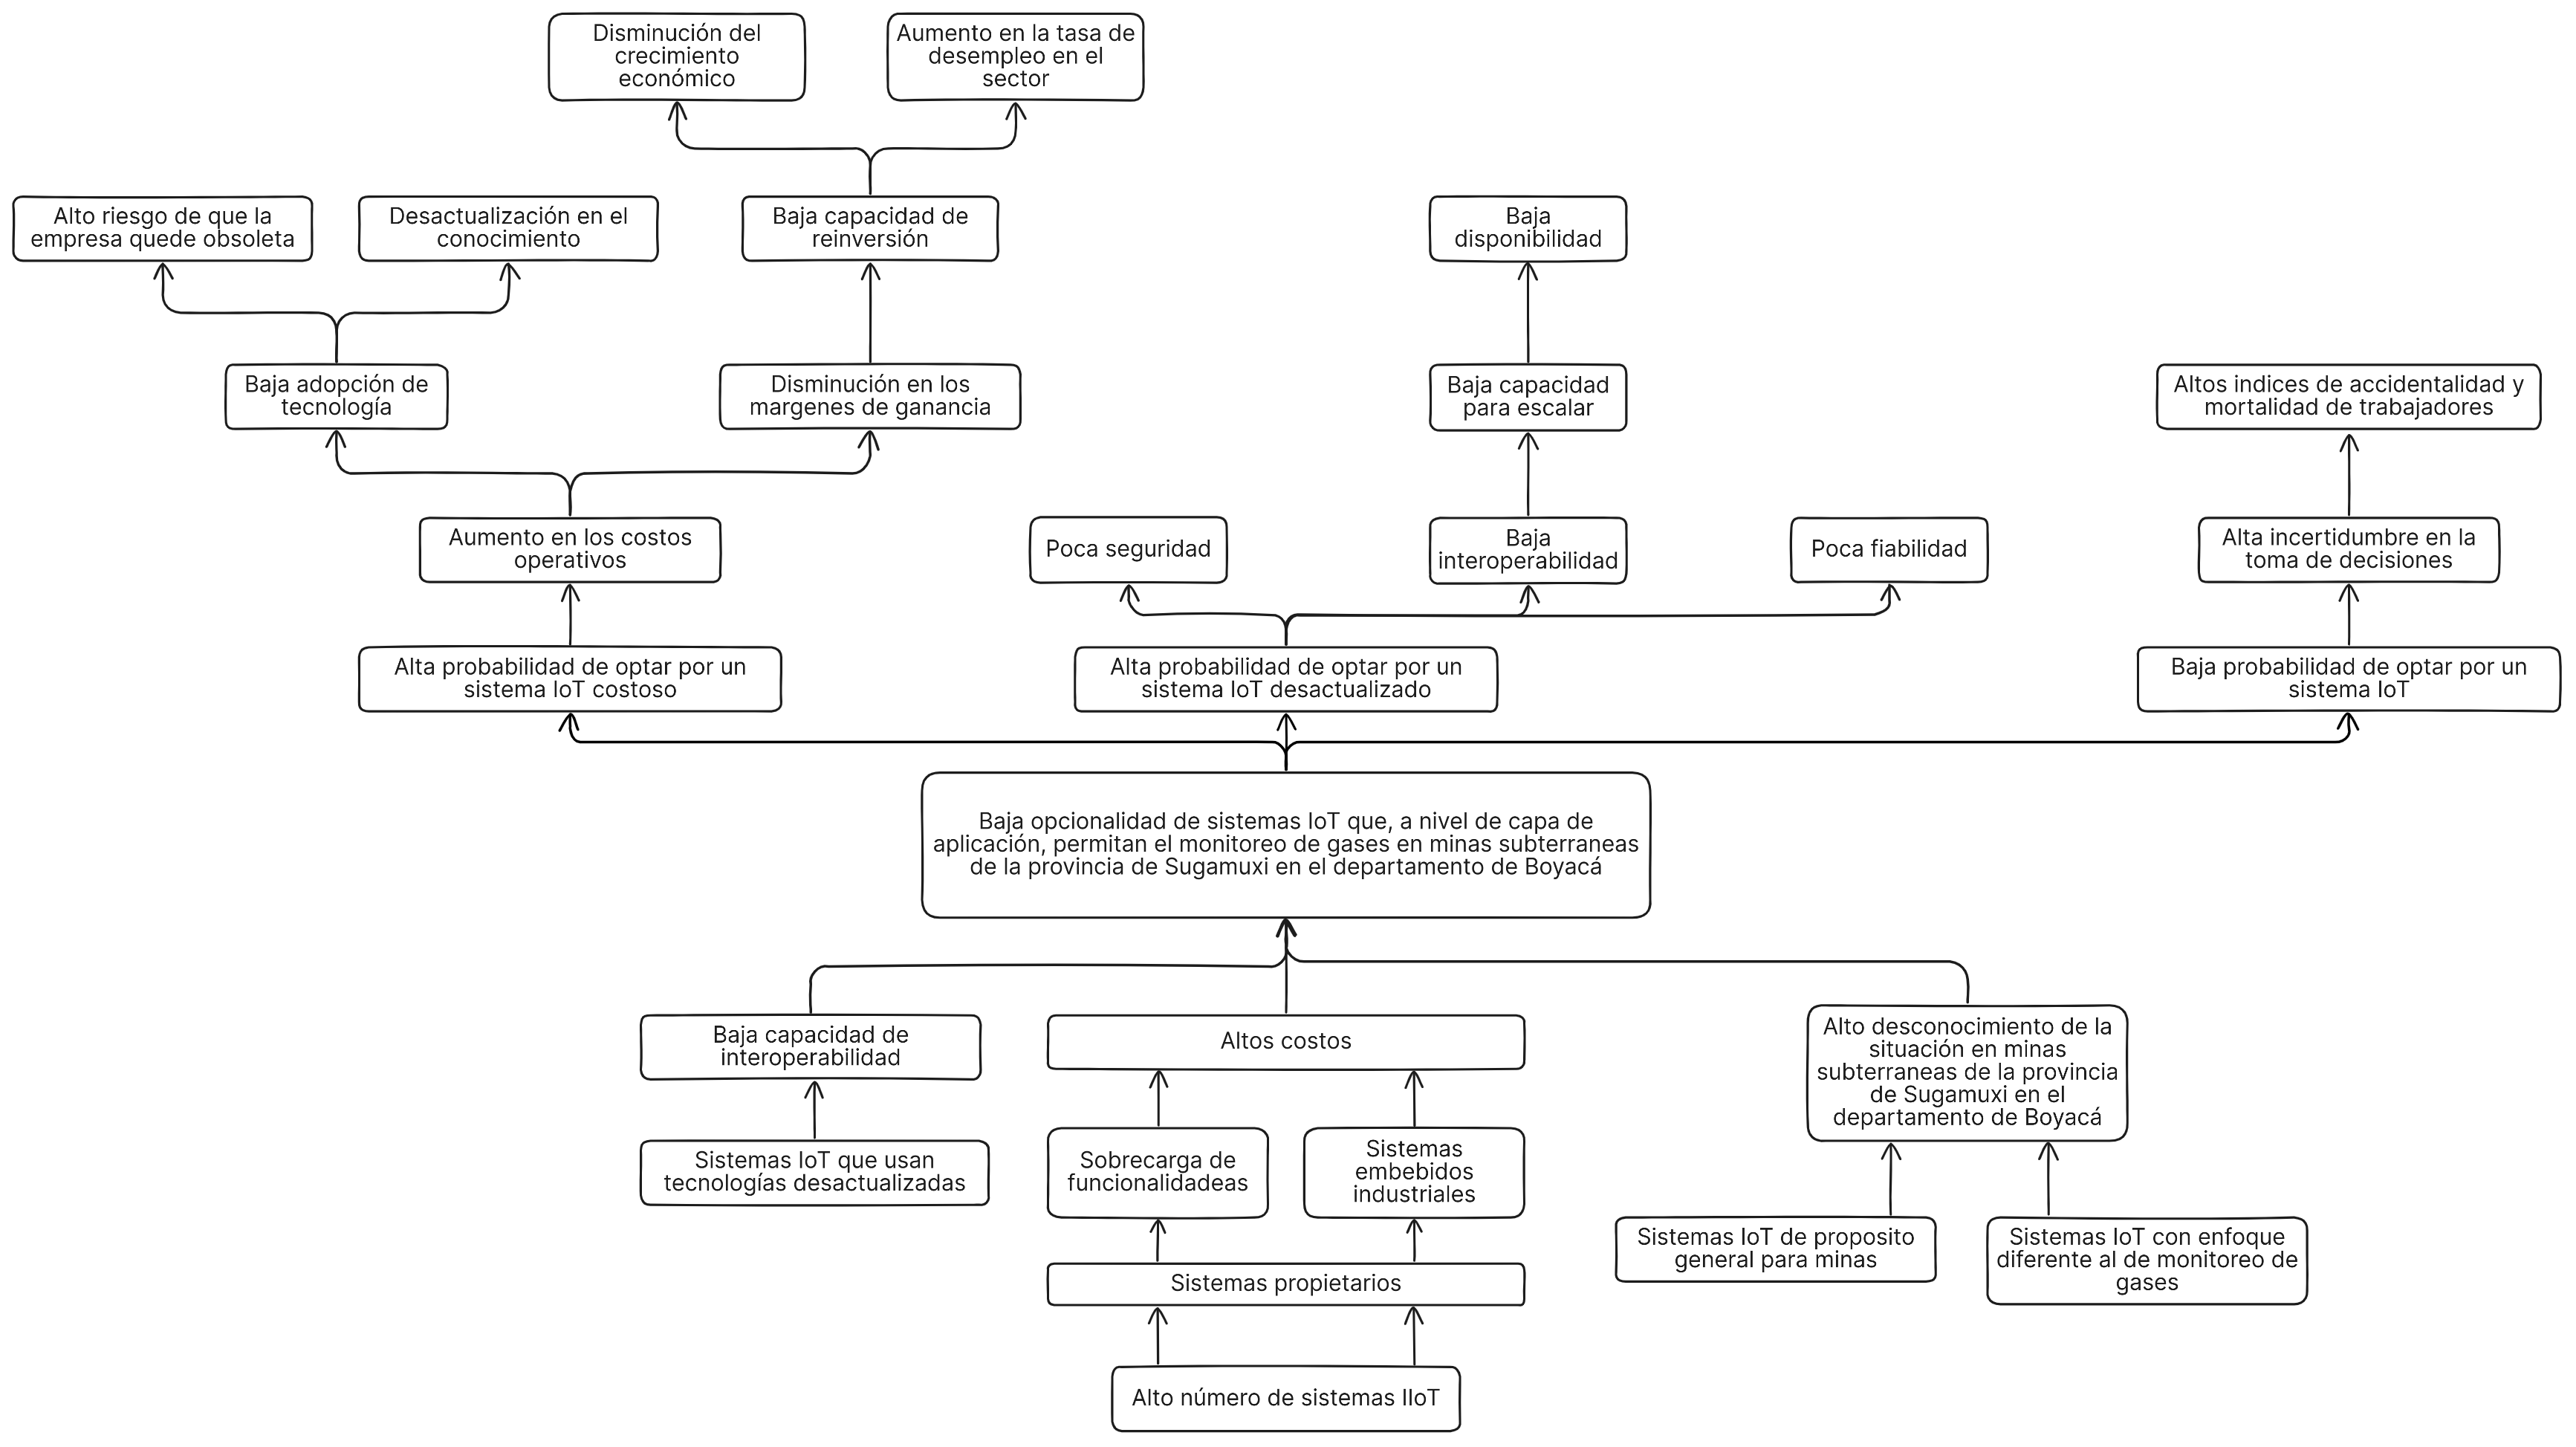
\includegraphics[scale=0.142]{arbol-causas-efectos}
		\captionsetup{justification=centering}
		\caption{Árbol de causas y efectos}
		\small
		Fuente: Autor
	\end{figure}
	
	\subsubsection{Control al pronostico}
	Ante la problemática planteada, surge la necesidad de disponer de un sistema IoT que, a nivel de capa de aplicación, cumpla con los siguientes atributos de calidad:
	
	\begin{itemize}
		\item Fiabilidad en la recolección de datos y emisión de alertas
		\item Disponibilidad 24/7
		\item Escabilidad principalmente asociada a la cantidad de datos que se recolectan por sistemas embebidos que amplíen los existentes.
		\item Mantenibilidad
		\item Seguridad principalmente en aspectos como la integridad, confidencialidad y disponibilidad de los datos.
		\item Rendimiento a nivel de recolección de datos y emisión de alertas
		\item Resiliencia 
		\item Monitoreo y diagnóstico
	\end{itemize}
	Además, es importante tener en cuenta que el sistema que se diseñe tiene que ser de bajo costo, por lo que va orientado al uso de sensores y actuadores de bajo costo también, específicamente de grado industrial. Lo anterior con el fin de que las minas de la provincia de Sugamuxi, Boyacá, puedan contar con una alternativa económicamente asequible sin perder los beneficios de un sistema IoT de calidad.
	\subsection{FORMULACIÓN DEL PROBLEMA}
	¿Qué aspectos se deben tener en cuenta para el diseño de la capa de aplicación de un sistema IoT que use una arquitectura de microservicios para el monitoreo de gases peligrosos en minas subterráneas de la provincia de Sugamuxi, Boyacá?
	%\begin{itemize}
		%   \item ¿Qué arquitecturas se encuentran consideradas en la industria minera para el desarrollo de sistemas IoT?
		   %\item ¿Cuáles son los estándares asociados a sistemas IoT en la industria minera?
			%\item ¿En qué aspectos la arquitectura de microservicios se presenta como una mejor opción frente a las demás arquitecturas planteadas para este contexto?
	%\end{itemize}
	
	\section{OBJETIVOS}
	\subsection{OBJETIVO GENERAL}
	Diseñar la capa de aplicación de un sistema IoT utilizando microservicios para el monitoreo de gases en minas subterráneas en la provincia de Sugamuxi, Boyacá, enfocado en la seguridad de las labores mineras.
	\subsection{OBJETIVOS ESPECÍFICOS}
	\begin{itemize}
		\item Analizar los diferentes modelos de transferencia de datos a nivel de capa de aplicación para sistemas IoT en entornos mineros.
		\item Identificar estándares en capa de aplicación asociados a sistemas IoT orientados al monitoreo de gases en entornos mineros.
		\item Clasificar y diseñar microservicios basados en las necesidades de seguridad y salud en el trabajo en minas de la provincia de Sugamuxi.
		\item Realizar pruebas de integración del sistema IoT para asegurar su funcionalidad y eficacia en el monitoreo de gases en entornos mineros.
	\end{itemize}
	\section{JUSTIFICACIÓN}
		%Por qué. De un conjunto de soluciones planteadas frente a una problematica, justificar, decir por qué se elige la solución n frente a las demás (ventajas, mejoras).
		%El conjunto de soluciones:
			%Sistemas desactualizados, podemos plantear mejoras a las falencias de estos
			%Sistemas que se pueden usar pero necesitan un enfoque al contexto de minas en la provinicia de Sugamuxi, Boyacá
			%Sistemas de alto costo, por el costo no podemos acceder a estos, pero podemos plantear una solución que tenga las funcionalidades y que debido al costo no pueden ser accedidas.
		
		La mayoría de plataformas mencionadas en tabla\ref{table:1}, a nivel de capa de aplicación, requieren que en las capas inmediatamente inferiores, del modelo de tres capas \ref{iot_tres_capas}, se haga uso de hardware propietario, principalmente sensores de categoría industrial que le elevan el costo de adquirir un sistema IoT. Otras de las plataformas mencionadas en el estudio carecen de capacidades requeridas para el monitoreo inteligente de gases, como lo son la analítica predictiva o la integración con sensores semi-industriales.
			
		
		%Para mitigar la carencia de sistemas desactualizados como el SCADA, muchas empresas en los últimos años han presentado al mercado soluciones basadas en IoT. Estas en su mayoría han probado ser opciones factibles debido a su uso por parte de empresas mineras grandes. Pero estas diferentes soluciones comparten la característica de tener pocos servicios, por lo que se tienen soluciones diferentes que no están en la capacidad de cubrir con todas las necesidades requeridas, como el procesamiento de datos por parte de algoritmos de ML sin tener que sacrificar aspectos como el almacenamiento y el acceso a estos. Además de que, como estas soluciones son concebidas en el contexto de empresas mineras de países desarrollados, es poco viable que una mina en un país en vía de desarrollo puede llegar a costearla. También es importante mencionar que muchas de las solucione implementadas son software de propietario, que fueron desarrollados por la empresa para la empresa\cite{iot-platforms}.
		
		%Para qué. Para mejorar, adquirir...
		  % Proveer una opción de bajo costo
		 Debido a la enorme cantidad de casos de uso de IoT, las arquitecturas varían entre diseños e implementaciones, por lo que se necesita tener presente las necesidades del contexto. Así que, partiendo de la concepción del modelo de tres capas\cite{10.1007/978-981-16-5655-2_3} se pretende diseñar la capa de aplicación del "Sistema IoT para el monitoreo de gases explosivos en minería subterránea", perteneciente al grupo de investigación GALASH de la UPTC Seccional Sogamoso.
		%A partir de esto, se identifica la necesidad de contar un sistema IoT con el enfoque de seguridad de las labores mineras, que cubra las necesidades especificas requeridas en el contexto de minas de la provincia de Sugamuxi en el departamento de Boyacá. Entre las que se encuentra el involucrar directamente a partes interesadas como los trabajadores y gerentes de minas, centros de atención a la salud que puedan responder a emergencias minimizando tiempos de respuesta, entidades gubernamentales como la Agencia Nacional Minera y el Ministerio de Minas y Energías. Planteando el diseño de un sistema IoT con el enfoque de seguridad de las labores mineras se le permite a estas partes interesadas el adquirir conocimiento de los diferentes aspectos requeridos en un sistema IoT .
		
		%Qué se busca. Validar, comprobar
		Con el desarrollo de la propuesta se quiere validar que se puede tener a disposición una solución que no implique costos elevados en comparación a las opciones anteriormente planteadas \ref{table:1}, comprobando que el software de uso libre es parte fundamental para lograrlo, sin tener que limitar las capacidades que un sistema IoT, en capa de aplicación, puede ofrecer.
	
		%Cómo se busca. Explicación paso a paso (metodologia)	
		Mediante la revisión de la literatura relacionada a diseño e implementación de sistemas IIoT en la industria minera, de uso y/o propósito general, arquitecturas de software y estándares relacionados, se pretende llegar a un consenso en el que se pueda producir un diseño que se ajuste a las necesidades planteadas por el contexto.
		
	\section{DELIMITACIÓN Y ALCANCE DE LA INVESTIGACIÓN}
	%Detalle puntualmente en párrafos de mínimo 5 líneas cada una de las siguientes delimitaciones:
	% - Por área geografica
	Siendo Boyacá uno de los departamentos con mayor tasa de accidentalidad y mortalidad en minas \cite{anm2020}, se pretende considera inicialmente a las minas subterráneas de carbón de la provincia de Sugamuxi, siendo el carbón el mineral más extraído en la provincia y estando la seccional Sogamoso territorialmente en la provincia de Sugamuxi también.
	
	%- Por recursos:
	Debido a la baja capacidad de inversión económica por partes de las minas de la provincia, el diseño tiene que ir orientado a minimizar costos.
	%- Por tecnología
	Para minimizar costos en la creación del diseño, se vuelve imperativo implementar herramientas de código abierto, pero sin comprometer la calidad de este.
	
	%Detalle puntualmente en párrafos de mínimo 5 líneas cada uno de los siguientes
	%alcances de la investigación en lo relacionado a:
	%- social,
	Se espera tener un impacto social ayudando a mejorar las condiciones laborales de los trabajadores de minas, especialmente de los involucrados directamente en la extracción de carbón. Llegando a proveer una opción que contribuya a disminuir los indices asociados a mortalidad  y accidentalidad 	minera en el departamento de Boyacá.
	%- humanístico,
	Al mejorar las condiciones laborales de los trabajadores se promueve el bienestar y la dignidad, reduciendo el riesgo asociado a sus actividades diarias dentro de las minas.
	%- educativo,
	
	Logrando un impacto social y humanístico es mucho más factible involucrar a diferentes instituciones educativas en el entendimiento de estas tecnologías, generando interés en las futuras generaciones, destacando la importancia de la minería para el departamento sin dejar de lado la seguridad de los involucrados en esta.
	%- religioso,
	%- cultural,
	Cuándo la comunidad pueda evidenciar que el uso de tecnología puede contribuir a la seguridad en el desarrollo de esta actividad, se puede cambiar la percepción de la minería como una actividad insegura, dando pie a más propuestas que encaminen a practicas modernas e innovadoras en la minería del departamento de Boyacá.
	%- Tecnologica
	
	El planteamiento de esta propuesta representa en algunos casos el punto de partida para otras, o el punto de integración de propuestas ya desarrolladas.
	%Hasta donde se llega en el proyecto
	Debido a que el diseño y desarrollo de un Sistema IoT involucra a profesionales de diferentes áreas del conocimiento, se parte del modelo comúnmente conocido de tres capas, para delimitar el alcance de este proyecto a la capa de aplicación
	
	\section{MARCO REFERENCIAL}
	\subsection{MARCO TEÓRICO}
	\subsubsection{Modelos  y Arquitecturas IoT}
	IoT (Internet of Things) no tiene una arquitectura estándar, a modo general se puede hablar de modelos para describir las diferentes arquitecturas que encontramos implementadas. Se describen modelos de tres capas\ref{iot_tres_capas}, cinco capas\ref{iot_cinco_capas} y siete capas\ref{iot_siete_capas}, pero en cuanto a la arquitectura de un sistema IoT las que sobresalen son implementadas por grandes empresas; Microsoft, Cisco, Amazon, Ericsoon, Intel, IBM, Google \cite{DBLP:journals/corr/abs-2004-12936}.
	
	La capa de aplicación del modelo de tres capas\ref{iot_tres_capas} aborda los servicios que serán usados por el usuario final. En cuanto a infraestructura, todo lo implementado en la capa de aplicación se encuentra en cloud.
	Para la capa red\ref{iot_tres_capas} se tiene contemplada la conexión entre las ''cosas'', los diferentes dispositivos de red y servidores, particularmente los desplegados en cloud.
	Finalmente en la capa de percepción\ref{iot_tres_capas} se encuentran los sensores y actuadores.
		\begin{figure}[H]
		\centering
		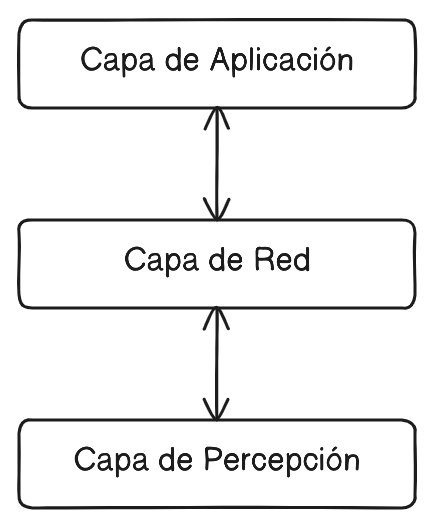
\includegraphics[scale=0.3]{iot_modelo_3_capas}
		\captionsetup{justification=centering}
		\caption{Modelo IoT de tre capas: Internet of Things Architectures: A Comparative Study}
		\small
		\label{iot_tres_capas}
		Adaptación de: Autor
	\end{figure}
	
	En el modelo de cinco capas se hace un análisis en el que da como resultado la especificación un poco más detallada de lo que sucede en capa de aplicación del modelo de tres capas\ref{iot_tres_capas}, dando como resultado la integración de dos capas más.. En la capa de negocio\ref{iot_cinco_capas} se gestiona y administra los dispositivos y software que se encuentra en las capas inferiores. En la capa de aplicación \ref{iot_cinco_capas} tenemos casi lo mismo que en la capa de aplicación del modelo de tres capas\ref{iot_tres_capas}. Siguiendo tenemos la capa de procesamiento\ref{iot_cinco_capas}, la cual se encarga de almacenar, analizar y procesar los datos recibidos por la capa inmediatamente inferior, esto a través del uso de bases de datos, computación en la nube, módulos de procesamiento de big data. La capa de transporte\ref{iot_cinco_capas} se encarga de la transferencia bidireccional de datos entre su capa inmediatamente superior e inferior. Finalmente para la capa de percepción de este modelo de cinco capas\ref{iot_cinco_capas} encontramos lo mismo que en la capa con el mismo nombre del modelo de tres capas\ref{iot_tres_capas}.
		\begin{figure}[H]
		\centering
		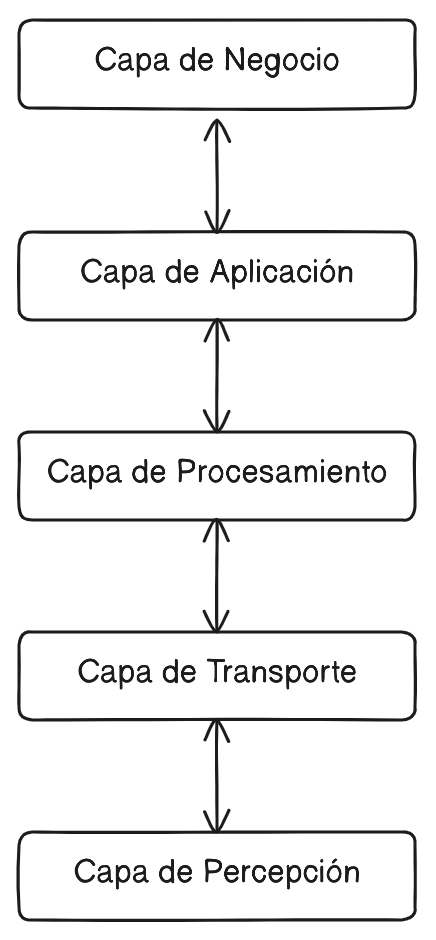
\includegraphics[scale=0.3]{iot_modelo_5_capas}
		\captionsetup{justification=centering}
		\caption{Modelo IoT de cinco capas: Internet of Things Architectures: A Comparative Study}
		\small
		\label{iot_cinco_capas}
		Adaptación de: Autor
	\end{figure}
	
	En el modelo de siete capas\ref{iot_siete_capas} iniciamos con la colaboración y procesos, en la que encontramos representados a los actores que usan los datos extraídos a través de las diferentes capas inferiores, para la toma de decisiones. En la capa de aplicación\ref{iot_siete_capas} están los usuarios que hacen uso de los datos extraídos por la demás capas inferiores, pero no hacen parte de la toma de decisiones de la organización que implementa el sistema IoT. Para la abstracción de datos\ref{iot_siete_capas}, estos son preparados para ser analizados por medio de técnicas de minado de datos y/o Machine Learning. En la acumulación de datos\ref{iot_siete_capas} se realiza almacenamiento con la garantía de que estos están siendo movidos de forma correcta. Cuando se hace referencia de Edge y/o Fog Computing\ref{iot_siete_capas}, se habla de la infraestructura usada para realizar transformación y análisis de datos antes de ser enviado a cloud. Finalmente en cuanto a conectividad\ref{iot_siete_capas} y  los dispositivos y controladores físicos se concibe prácticamente lo mismo que en los dos modelos anteriores.
	
		\begin{figure}[H]
		\centering
		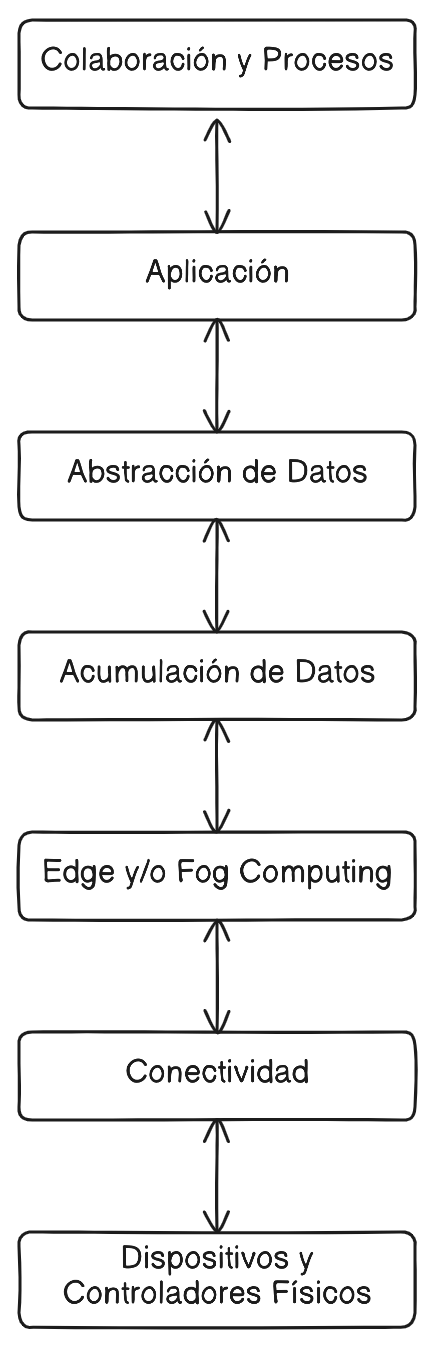
\includegraphics[scale=0.3]{iot_modelo_7_capas}
		\captionsetup{justification=centering}
		\caption{Modelo IoT de siete capas: Internet of Things Architectures: A Comparative Study}
		\small
		\label{iot_siete_capas}
		Adaptación de: Autor
	\end{figure}
	
	\subsubsection{IIoT en la industria minera}
	IoT en la industria minera representa el medio para la operación y monitoreo remoto de sistemas de producción complejos en los que se minimiza la intervención completa y/o parcial humana, haciendo uso de plataformas en tiempo real\cite{molaei:hal-02940030}.
	
	La arquitectura que aparece en la figura\ref{iiot_minas_arq_sintetizada}, resultado del estudio de  \cite{iot1020029}, nos da una vista bastante buena de los diferentes aspectos que se ven involucrados dentro de una arquitectura IIoT orientada a la industria minera, clasificando por dominios y diferenciando estos por su implementación en el sitio minero o fuera de este, ubicándolos a nivel de infraestructura en lo que se conoce como ''Computación Niebla" por su traducción del inglés Fog Computing y ''Computación en la Nube" por su traducción del inglés Cloud Computing.
		\begin{figure}[H]
		\centering
		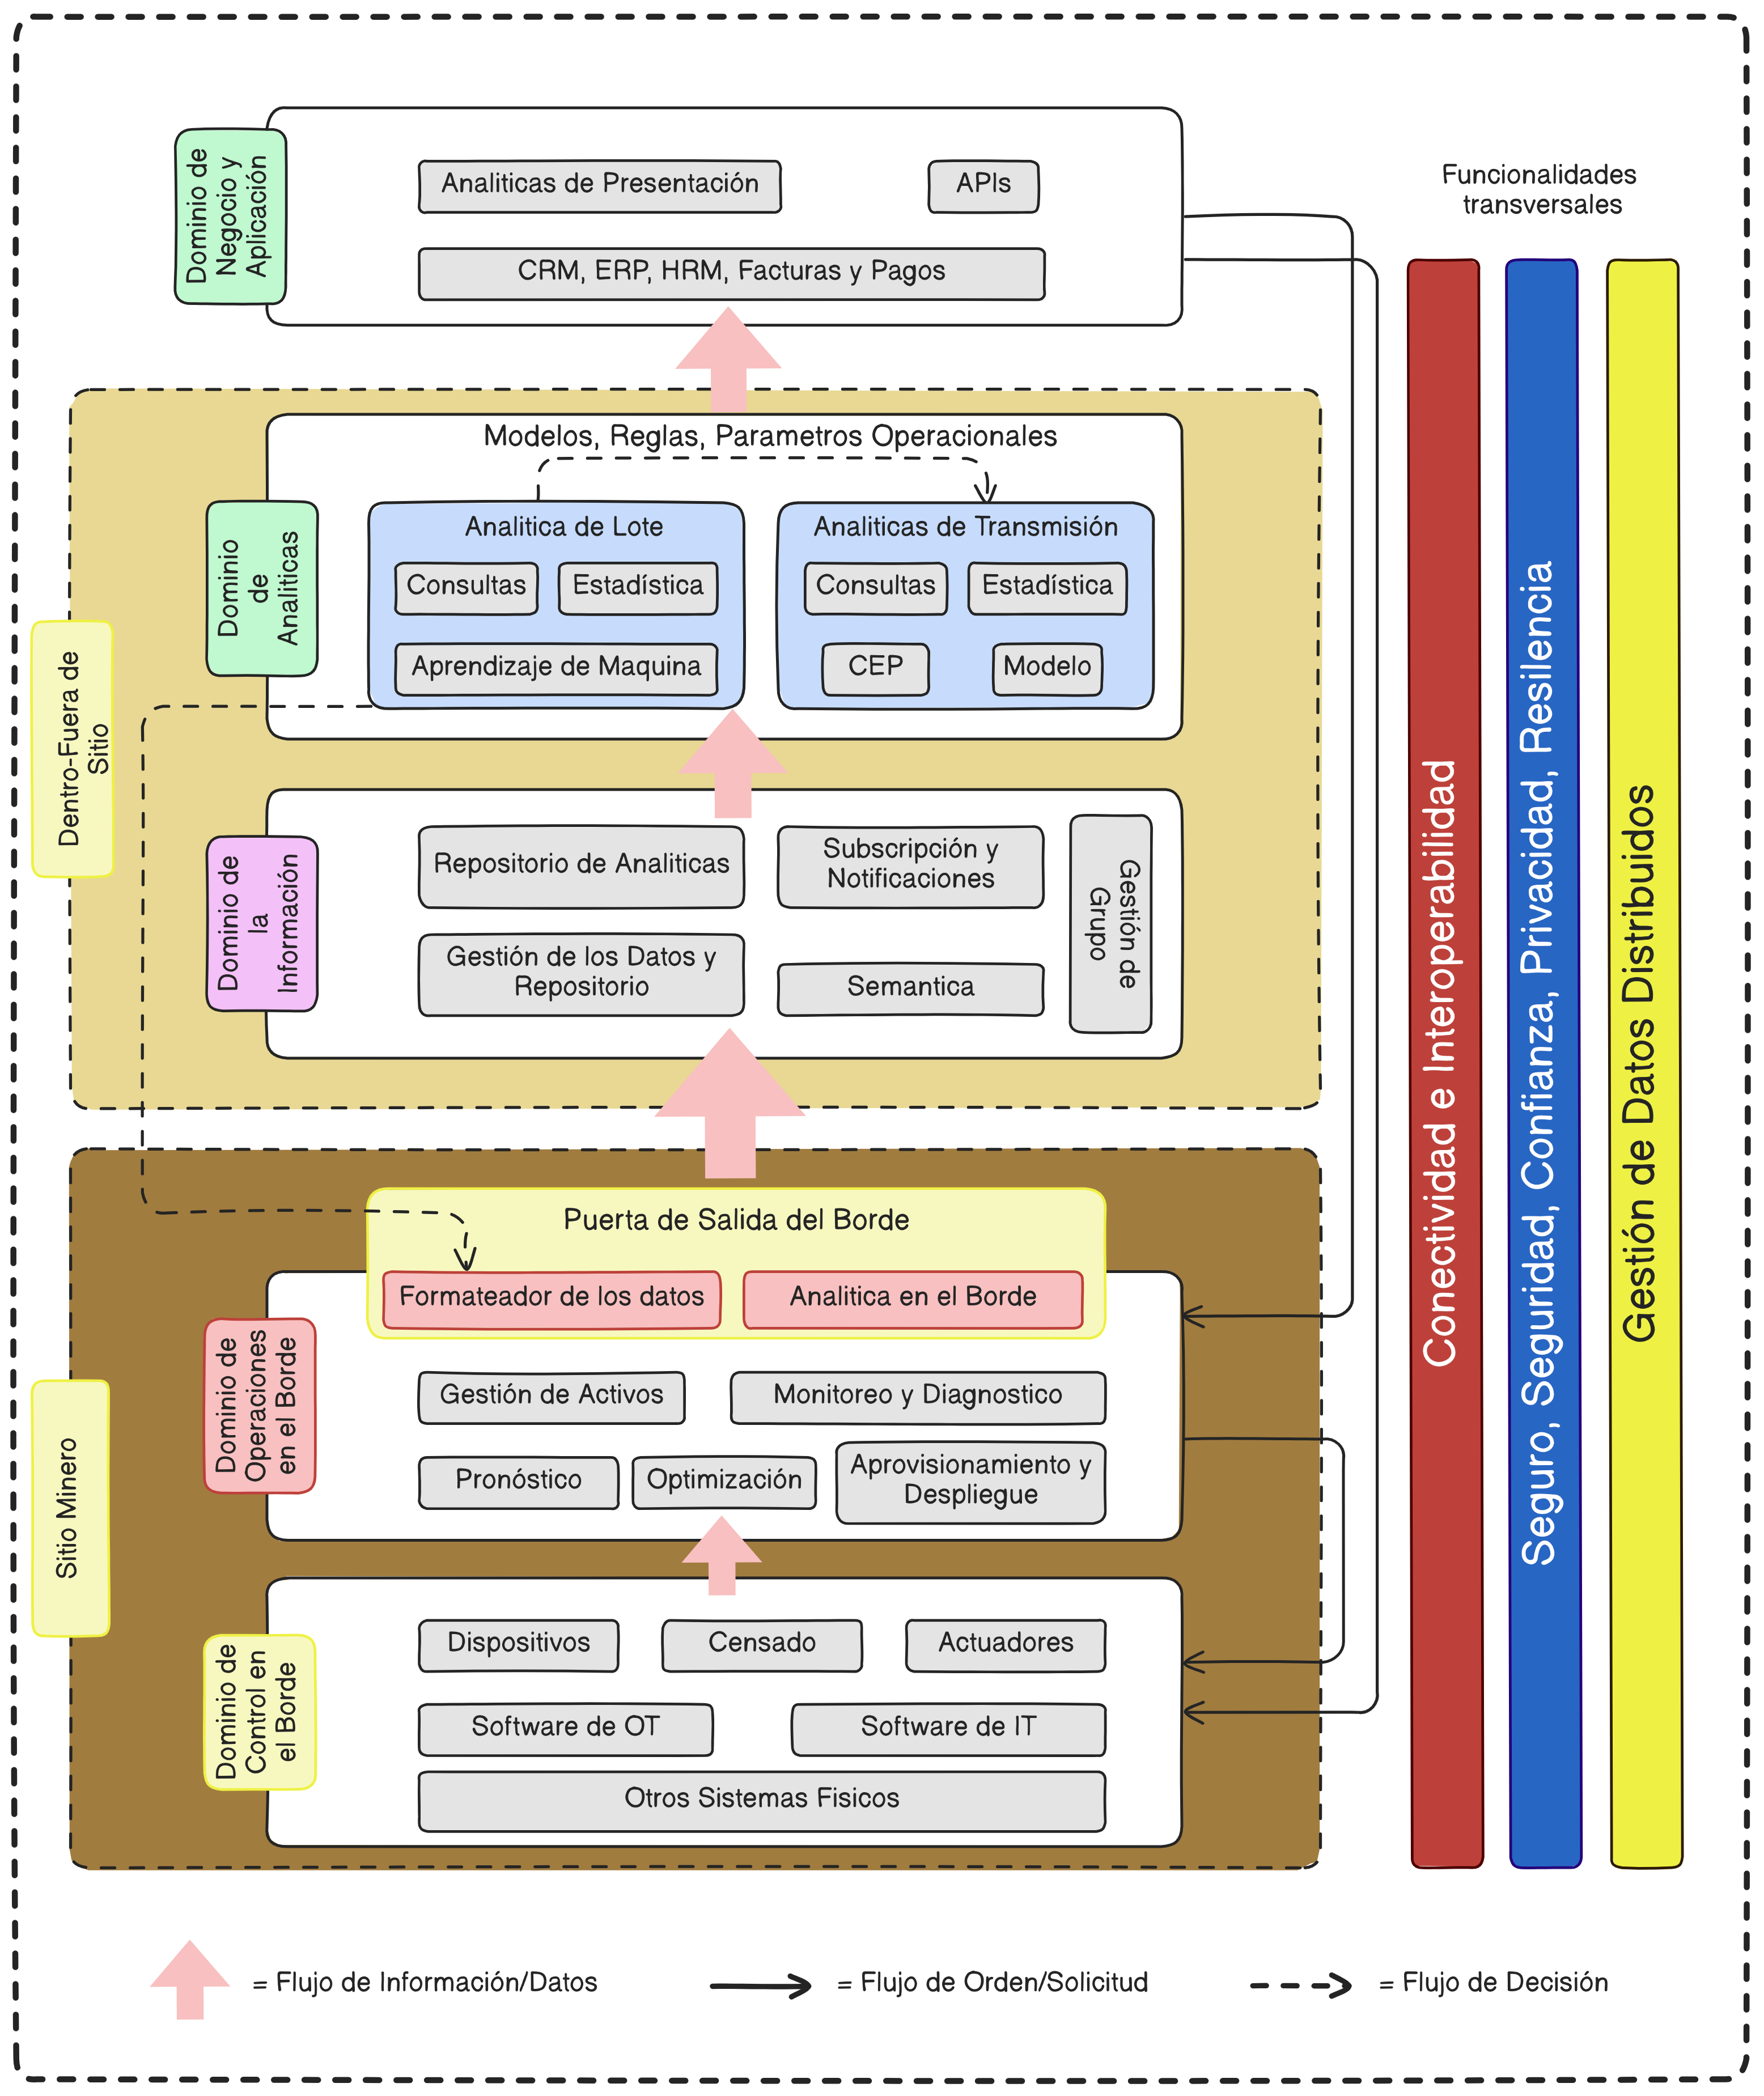
\includegraphics[scale=0.13]{Adaptacion_Synthesized_high_level_IIoT_architecture_for_mining_industry.png}
		\captionsetup{justification=centering}
		%\caption{Synthesized high level IIoT architecture for mining industry}
		\caption{Arquitectura IIoT sintetizada a nivel genera para la industria mineral}
		\small
		\label{iiot_minas_arq_sintetizada}
		Adaptación de: Autor
	\end{figure}
	\subsubsection{Protocolos de comunicación en IoT para capa de aplicación}
	%Paper 1 sobre protocolos \cite{en13112762}
	En IoT existe una gran variedad de protocolos que van desde la capa más baja de cualquier modelo hasta la de más alto nivel, que en este caso entendemos como capa de aplicación. En capa de aplicación, la clasificación de estos se puede hacer varias formas, pero una distinción común que se hace entre la gran variedad de protocolos, ya poniendo la en términos de costos, es la de diferenciar a estos en protocolos de uso libre y protocolos propietarios [insertar cita].
	Indiferentemente de lo anterior, para capa de aplicación de IoT, se encuentran entre los más conocidos; MQTT, AMQP, CoAP, XMPP y DDS \cite{YUGHA2020102763}.
	\begin{enumerate}[label=\alph*)]
	\item MQTT: De sus siglas en inglés Message Queue Telemetry Transport (MQTT) y de su traducción al español "Transporte de Telemetría de Cola de Mensajes", es un protocolo ampliamente usado desde su desarrollo en 1999, con características como su diseño orientado a mensajes livianos, siguiendo el modelo de cliente-servidor, en el que el cliente pude tomar el rol de publicador o suscriptor y el servidor cumple el rol de "Broker", encargándose del transporte de mensajes entre y para clientes publicadores y suscriptores \cite{EEI5236}.
	\item AMQP: De sus siglas en inglés Advance Message Queuing Protocol (AMQP) y de sus traducción al español "Protocolo Avanzado de Cola de Mensajes", es un protocolo centrado u orientado a los mensajes, proveyendo intercambio de mensajes a través de los roles de publicador y suscriptor \cite{YUGHA2020102763}.
	\item CoAP: De sus siglas en inglés Constrained Application Protocol (CoAP) y de sus traducción al español "Protocolo de Aplicación Restringido", es un protocolo que que usa la arquitectura cliente-servidor, similar a HTTP pero usando como protocolo de transporte UDP en lugar de TCP presente en HTTP \cite{YUGHA2020102763}.
	\item XMPP: De sus siglas en inglés Extensible Messaging and Presence Protocol (XMPP) y de su traducción al español "Protocolo Extensible de Mensajería y Presencia", es un protocolo basado en  Extensible Markup Language (XML) y que usa TCP como protocolo de transporte. La transmisión de mensajes es distribuida y no centralizada como es el caso de MQTT o AMQP \cite{YUGHA2020102763}.
	\item DDS: De sus siglas en inglés Data Distribution Service (DDS) y de su traducción al español, "Servicio de Distribución de Datos", es usado para comunicaciones de punto a punto para dispositivos IoT de baja latencia \cite{YUGHA2020102763}.
	\end{enumerate}
	%\subsubsection{IoT para el monitoreo de gases}
	
	%\subsubsection{Infraestructura IoT}
	
	%\subsubsection{Machine Learning para IoT}
	
	%\subsubsection{Ingeniería de Software}
	
	\subsubsection{Arquitectura de Microservicios}
	La arquitectura de Microservicios, predecesora en orden cronológico de concepción de la Arquitectura Orientada a Servicios por sus siglas en inglés Services Oriented Architecture (SOA), se puede entender como el conjunto de servicios granulares desplegados en diferentes stacks tecnológicos que en conjunto, a través de uno o varios protocolos de comunicación, logran interacción en beneficio de un sistema o software \cite{WASEEM2020110798}.
	
	En el estudio de \cite{10220070} sobre arquitectura de microservicios, se encuentran identificadas unas series de practicas, patrones y principios resumidos en \ref{tabla_resumen_microservicios} y que se dedujeron a través de la revisión de documental de arquitecturas de microservicios implementadas por parte de diferentes empresas.
	

	\begin{longtable}{ | >{\centering\arraybackslash}p{3cm} | >{\centering\arraybackslash}p{3cm} | >{\centering\arraybackslash}p{3cm} | >{\centering\arraybackslash}p{3cm} | }
		\hline
		\thead{\textbf{Nombre}} & \thead{\textbf{Intención}} & \thead{\textbf{Escenario de uso}} & \thead{\textbf{Beneficios clave}} \\
		\hline
		\endfirsthead
		
		\hline
		\thead{\textbf{Nombre}} & \thead{\textbf{Intención}} & \thead{\textbf{Escenario de uso}} & \thead{\textbf{Beneficios clave}} \\
		\hline
		\endhead
		
		\hline
		\endfoot
		
		\hline
		\caption{\centering Resumen de metodologías y patrones para microservicios\\ Adaptación de: Autor\\}
		\label{tabla_resumen_microservicios}
		\endlastfoot
		
		Diseño Orientado al Diseño & Diseñar y desarrollar sistemas de software con base en el modelo del dominio & Dominios complejos con lógica de negocio rica y en evolución & Alineamiento claro con el dominio, encapsulamiento del conocimiento del dominio, diseño modular y con mantenibilidad, mejora la colaboración entre equipos \\
		\hline
		Patrón de Descubrimiento de Servicio & Facilita el descubrimiento y la comunicación de servicios dinámicos & Arquitecturas de Microservicios con interacción de servicios & Registro dinámico y automático de servicios, desacoplamiento entre servicios, balanceo de cargas, tolerante a fallos\\
		\hline
		Diseño Orientado a los Datos&Diseñar sistema de software al rededor del comportamiento y estructura de los datos & Aplicaciones donde los datos son un componente clave& Enfocado en la toma de decisiones orientadas a los datos, mejora la integridad de los datos, optimiza el acceso y la manipulación de los datos, alineado con objetivos del negocio \\
		\hline
		Patrón de Backend para Frontend& Desarrollar servicios de backend hecho a la medida de ciertos clientes frontend&Aplicaciones con múltiples clientes de frontend& APIs customizadas y optimizadas para cada cliente de frontend, desacoplamiento de frontend-backend mejorado, una mejor experiencia de usuario \\
		\hline
		Patrón Adaptador de Microservicios&Adapta y transforma datos o funcionalidad entre microservicios&Arquitecturas de Microservicios con diferentes interfaces&Permite una comunicación fluida entre microservicios con diferentes protocolos o formato de datos, promueve la interoperabilidad\\
		\hline
		Patrón de Aplicación Estrangulador&Migrar incrementalmente de un sistema monolítico a microservicios & Aplicaciones monolíticas antiguas, desactualizadas, obsoletas & Migración gradual sin de perturbar el sistema existente, riesgo reducido, mantenibilidad y escalabilidad mejoradas\\
		\hline
		Patrón de diseño de microservicio de datos compartidos&Gestiona y comparte datos entre microservicios &Arquitecturas de Microservicios con requerimientos para compartir datos&Gestión centralizada de datos, consistencia de datos, duplicación y redundancia de datos reducida, integridad de los datos mejorada\\
		\hline
		Patrón de diseño de microservicio de agregador o consolidación&Datos consolidados o agregados, o funcionalidades desde múltiples microservicios&Aplicaciones que requieren información consolidada& Agregación o consolidación de datos centralizados, complejidad del cliente reducida, mejora el rendimiento, sobrecarga de la red reducida\\
		\hline
		% Añade tantas filas como necesites
		
	\end{longtable}
	%\subsubsection{Protocolos de comunicación para microservicios}
	
	%\subsubsection{Software orientado a capa de aplicación de IoT}
	
	\subsection{MARCO CONCEPTUAL}
		\begin{itemize}
		\item IoT (Internet of Things): Por su traducción al español "Internet de las Cosas", se entiende como una red global de dispositivos "inteligentes" (principalmente de baja capacidad computacional) interconectados entre sí a través de internet.
		\item IIoT (Industrial Internet of Things): Por su traducción al español "Internet de las Cosas en la Industria", es una aplicación o caso de uso de IoT en la industria.
		\item Nodos sensores: Dispositivos que, siguiendo el modelo de tres capas de un arquitectura IoT, se encuentran en la capa de percepción y se encargan de recolectar información sobre su entorno.
		\item Gateway IoT: Componente de un Sistem IoT encargado de dotar a los nodos sensores de la capacidad de "salir a internet", además de otras capacidades como seguridad, analítica.
		\item Computación en la nube (Cloud computing): Infraestructura computacional perteneciente a un tercero en la mayoría de los casos, pero con la característica principal de estar ubicada a cientos de kilómetros del dominio o sitio dónde se generan los datos y/o acciones.
		\item Computación en el borde (Edge Computing): Infraestructura computacional que se encuentra en el sitio donde se generan los datos y/o acciones.
		\item Computación niebla (Fog Computing): Infraestructura que no se puede clasificar como Edge ni como Cloud.
		\item Monitoreo de condiciones ambientales: Percepción de variables del entorno a través de dispositivos de sensado para la toma de decisiones.
		\item Monitoreo fisiológico %Monitoreo de personal
		\item Tecnología Operacional (Operational Technology)
		\item Tecnología de la Información (Information Technology)
		\item Interoperabilidad: Capacidad de comunicación entre diferentes sistemas para el intercambio de información.
		\item Semántica de los Datos: Metadatos y contexto que describen lo que representan los datos, cómo se deben interpretar y se relacionar entre si.
		\item Provisión de los Datos: Proceso de preparación y suministración de datos a los diferentes usuarios y/o aplicaciones que los requieren.
		\item Análisis Predictivo: Tipo de análisis orientado a la toma de decisiones antes de que un suceso ocurra.
		\item Machine Learning: 
		\item Visualización de Datos Avanzados
		\item Captura de Datos en Tiempo Real
		\item Gestión de Dispositivos de Forma Remota
		\item Arquitectura IoT
		\item Capa de Aplicación en una Arquitectura IoT
		\item Capa de Red en una Arquitectura IoT
		\item Capa de Percepción en una Arquitectura IoT
	\end{itemize}
	\subsection{MARCO LEGAL}
	Normas ATEX
	
	Ley 1581 de 2012 de la protección de datos personales en Colombia
	
	Decreto 1377 de 2013
	\subsection{MARCO HISTÓRICO}
	SCADA → M2M → IoT
	
	Los sistemas IIoT (Industrial Internet of Things) como una aplicación de IoT (Internet of Things) en la industria, hacen uso de sistemas IoT para el monitoreo de condiciones ambientales, en el caso de la industria minera por medio de sensores para la calidad del aire, la detección de gases nocivos para la salud, así como para la detección de partículas de polvo producidos principalmente en el proceso de extracción de minerales, se pretende garantizar información principalmente en tiempo real que ayude a la toma de decisiones de prevención y gestión de emergencias\cite{reference-1}.
	%con las características claves  de interfaz de usuario, pantallas gráficas, alarmas, tendencias, interfaces RTU (Unidades Terminales Remotas) y PLC (Controladores Lógicos Programables), escalabilidad, acceso a datos, bases de datos, redes, tolerancia a fallos y redundancia, procesamiento distribuido siguiendo la arquitectura cliente/servidor. 
	SCADA, ha servido en el proceso de recolección y procesamiento de datos a nivel general en la industria por varias décadas. Los sistemas SCADA, principalmente los implementados años atrás, presentan baja capacidad de interoperabilidad con otras partes interesadas como lo son otros sistemas, dispositivos, aplicativos usados por stakeholders \cite{SCADA_UMaT}.
	
	\section{FUENTES DE INFORMACIÓN}
	\subsection{Fuentes primarias}
	El formato de estos será en su mayoria el distribuido electronicamente, a no ser que se requiera un libro que por ciertas circunstancias se encuentre solamente en formato tradicional impreso. En cuanto al dónde encontrar estas fuentes, siendo en su mayoría electronicas, se primara el uso de buscadores o indexadores de articulos de investigación, bibliotecas en linea, tiendas en linea, catalogos.
	
	Por consecuencia, como fuentes de información primaria se tendrán obras literias, reportes de investigación, normas tecnicas, tesis, revistas cientificas,  articulos que empiecen manejando como parte fundamental de este el uso, diseño, implementación de IoT
	\subsection{Fuentes secundarias}
	Revistas puestos a trabajo de revisión, informes de investigación
	%\subsection{Fuentes terciarias}
	\section{MARCO METODOLÓGICO}
	\subsection{Tipo de investigación}
	Investigación comparada
	% Investigación de acción participativa? Porque puede ser relevante para este caso conocer de primera mano la opinion de las partes interesadas.
	\subsection{Alcance de la investigación}
	Experimental
	\subsection{Enfoque de la investigación}
	Mixto
	\subsection{Metodología de desarrollo}
	Metodología ágil
	%\subsection{Población y muestra}
	%Sistemas IoT en la industria y Sistemas IoT para el monitoreo de gases
	
	%Minas de Colombia → Minas subterráneas de carbón de la provincia de Sugamuxi, Boyacá.
	%\subsection{Instrumentos de recolección de datos}
	%Diagrama de flujo
	\section{CRONOGRAMA}
		\begin{figure}[H]
		\centering
		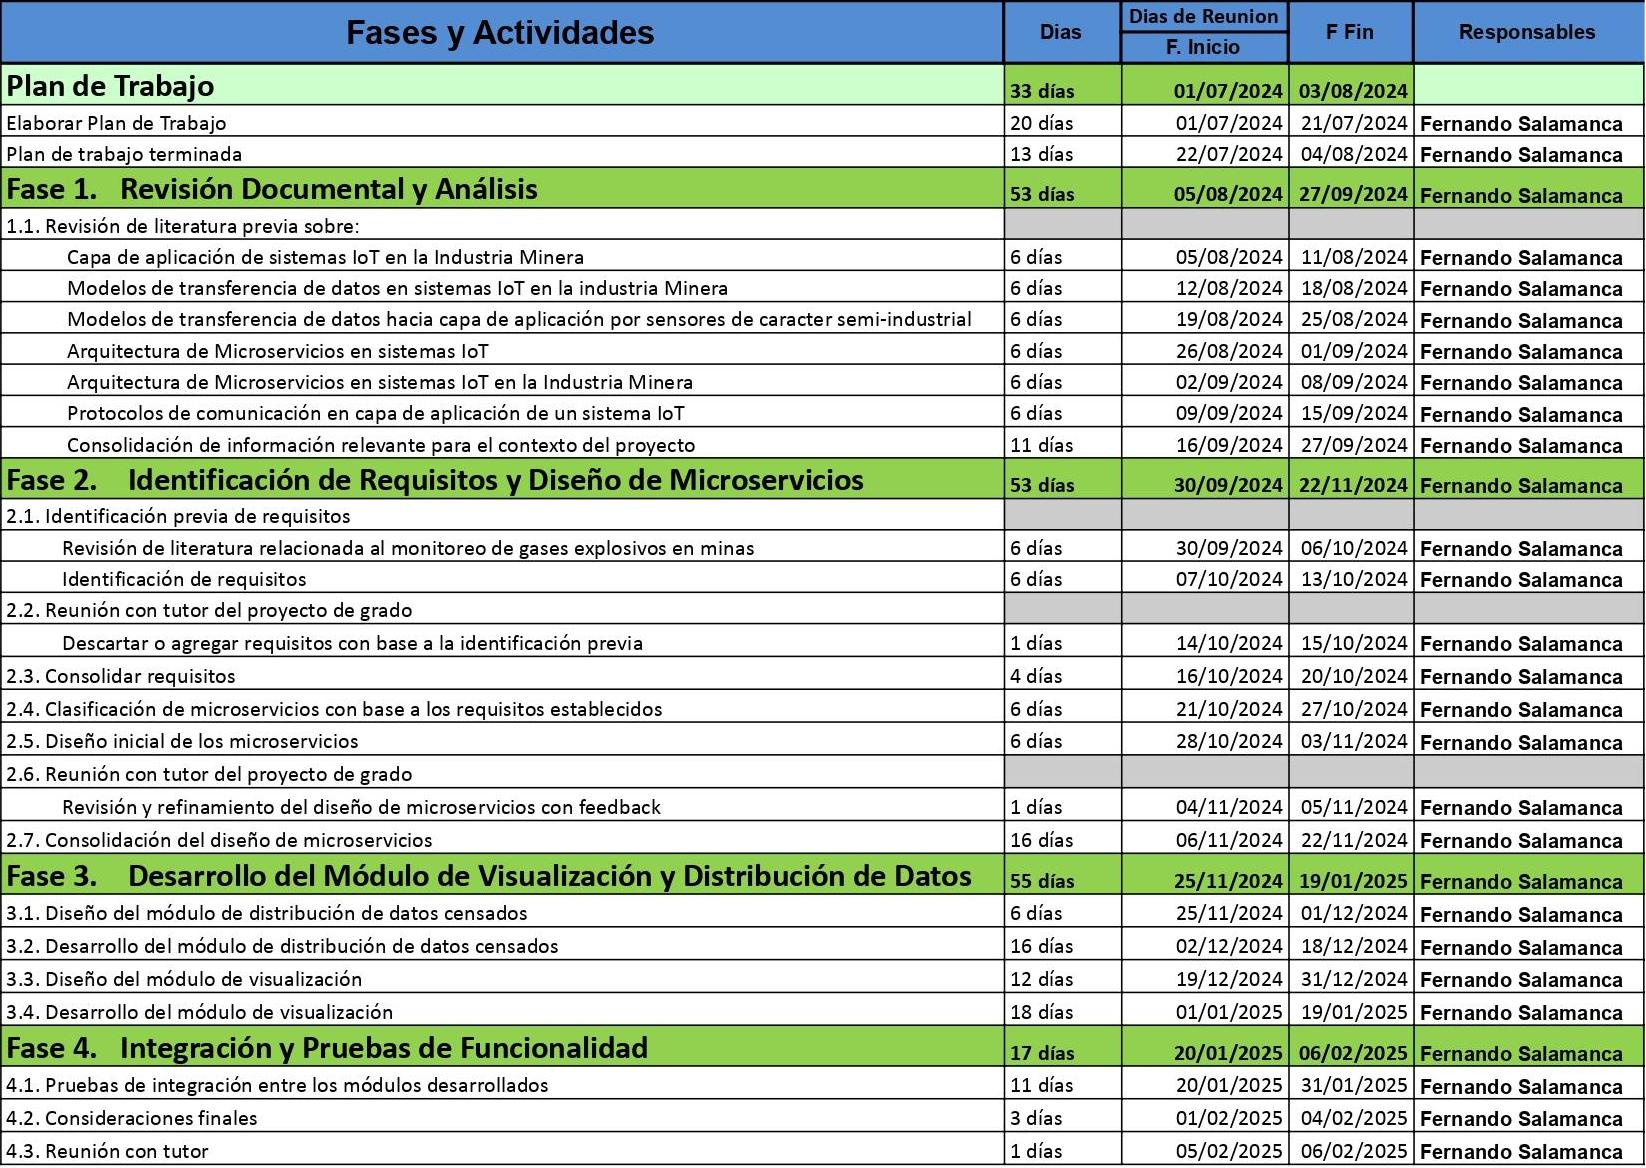
\includegraphics[scale=0.6]{cronograma.jpg}
		\captionsetup{justification=centering}
		\caption{Cronograma del Proyecto}
		\small
		\label{cronograma}
	\end{figure}
	\section{RECURSOS}
	\subsection{RECURSOS HUMANOS}
	\subsection{RECURSOS FÍSICOS}
	\subsection{RECURSOS TECNOLÓGICOS}
	
	\section{PRESUPUESTO}
	\section{CONCLUSIONES}
	\section{BIBLIOGRAFÍA}
	\renewcommand\refname{Referencias}
	\bibliographystyle{apalike}
	\bibliography{./references.bib}
\end{document}
